\documentclass[
    11pt,
    a4paper
]{article}

% =========================================================
% IDIOMA, CODIFICACIÓN Y TIPOGRAFÍA
% =========================================================

\usepackage[utf8]{inputenc}
\usepackage[T1]{fontenc}
\usepackage{csquotes}
\usepackage[french]{babel}
\usepackage{lmodern}

% =========================================================
% GEOMETRÍA DE LA PÁGINA
% =========================================================

\usepackage[
    top=2.5cm,
    bottom=2.5cm,
    left=2.8cm,
    right=2.8cm
]{geometry}

% =========================================================
% MATEMÁTICAS
% =========================================================

\usepackage{amsmath}
\usepackage{amssymb}
\usepackage{amsfonts}
\usepackage{mathtools}
\usepackage{bm}

% =========================================================
% UNIDADES Y NOTACIÓN CIENTÍFICA
% =========================================================

\usepackage{siunitx}

\sisetup{
    output-decimal-marker={,},
    separate-uncertainty=true,
    per-mode=symbol
}

% =========================================================
% FIGURAS
% =========================================================

\usepackage{graphicx}
\usepackage{float}
\usepackage{subcaption}
\usepackage{placeins}

% Carpeta compartida (misma para todas las etapas) donde Etapa_2.py y demas scripts
% guardan sus figuras -- ver PLOTS_DIR en Etapa_2.py
\graphicspath{{../plots/}}

% =========================================================
% TABLAS
% =========================================================

\usepackage{booktabs}
\usepackage{tabularx}
\usepackage{array}
\usepackage{multirow}
\usepackage{longtable}

% =========================================================
% COLORES
% =========================================================

\usepackage{xcolor}

\definecolor{linkcolor}{RGB}{0,70,140}
\definecolor{citecolor}{RGB}{0,100,70}
\definecolor{urlcolor}{RGB}{120,40,120}

% =========================================================
% HIPERVÍNCULOS Y REFERENCIAS CRUZADAS
% =========================================================

\usepackage[
    colorlinks=true,
    linkcolor=linkcolor,
    citecolor=citecolor,
    urlcolor=urlcolor,
    bookmarksopen=true,
    bookmarksnumbered=true
]{hyperref}

\usepackage[nameinlink, noabbrev]{cleveref}

\crefname{equation}{équation}{équations}
\Crefname{equation}{Équation}{Équations}

\crefname{figure}{figure}{figures}
\Crefname{figure}{Figure}{Figures}

\crefname{table}{tableau}{tableaux}
\Crefname{table}{Tableau}{Tableaux}

\crefname{section}{section}{sections}
\Crefname{section}{Section}{Sections}

\crefname{subsection}{sous-section}{sous-sections}
\Crefname{subsection}{Sous-section}{Sous-sections}

% =========================================================
% ENCABEZADOS Y PIES DE PÁGINA
% =========================================================

\usepackage{fancyhdr}

\pagestyle{fancy}
\fancyhf{}

\fancyhead[L]{Convergence de la limite de stabilité selon la taille de dexel (Étape 2)}
\fancyhead[R]{\thepage}
\setlength{\headheight}{14.2pt}

\renewcommand{\headrulewidth}{0.4pt}
\renewcommand{\footrulewidth}{0pt}

% =========================================================
% FORMATO DE TÍTULOS
% =========================================================

\usepackage{titlesec}

\titleformat{\section}
    {\Large\bfseries}
    {\thesection.}
    {0.5em}
    {}

\titleformat{\subsection}
    {\large\bfseries}
    {\thesubsection.}
    {0.5em}
    {}

% =========================================================
% ESPACIADO
% =========================================================

\usepackage{setspace}

\setstretch{1.15}
\setlength{\parindent}{0pt}
\setlength{\parskip}{0.6em}

% =========================================================
% BIBLIOGRAFÍA
% =========================================================

\usepackage[
    backend=biber,
    style=numeric,
    sorting=none
]{biblatex}

\addbibresource{references.bib}

% =========================================================
% MICROTIPOGRAFÍA
% =========================================================

\usepackage[patch=none]{microtype}

% =========================================================
% COMANDOS PERSONALIZADOS
% =========================================================

\newcommand{\ap}{a_p}
\newcommand{\apcrittheo}{a_{p,\mathrm{crit,theo}}}
\newcommand{\apcritsim}{a_{p,\mathrm{crit,sim}}}
\newcommand{\dxlsize}{\Delta_{\mathrm{dxl}}}
\newcommand{\etac}{\eta_{\mathrm{crit,sim}}}

% =========================================================
% INFORMACIÓN DEL DOCUMENTO
% =========================================================

\title{
    \textbf{Influence de la taille de dexel sur la limite de stabilité simulée (Étape 2)}
}

\author{
    Enrique Mireles
}

\date{\today}

% =========================================================
% INICIO DEL DOCUMENTO
% =========================================================

\begin{document}

\maketitle

\begin{abstract}

Ce document étudie l'influence de la taille de dexel \(\dxlsize\) sur la limite de
stabilité \(\apcritsim\) détectée par simulation, dans le modèle dynamique le plus simple
du pipeline (profondeur axiale \(\ap\) constante, \enquote{modèle tube}), en reprenant la
méthode de bissection de l'Étape~1 pour neuf tailles de dexel réparties autour de la valeur
de base retenue à l'Étape~0. L'objectif est de déterminer si \(\apcritsim\) converge vers la
valeur théorique \(\apcrittheo\) lorsque \(\dxlsize\) diminue, ou si elle continue de dériver
sans convergence -- le doute qui a motivé le réagencement complet du travail en étapes
isolant chacune un paramètre. Les résultats montrent une convergence rapide de
\(\apcritsim\) vers \(\apcrittheo\) (écart de l'ordre de \SI{1}{\percent} à \SI{2}{\percent})
sur la majeure partie du balayage, la taille de dexel n'ayant qu'une influence négligeable
sur la détection de l'instabilité dans ce modèle simplifié -- à l'exception du dexel le plus
grossier du balayage, pour lequel la détection se dégrade nettement.

\end{abstract}

\tableofcontents

\newpage

\section{Introduction}
\label{sec-introduction}

L'Étape~1 a établi, pour une taille de dexel fixe \(\dxlsize = 2\times10^{-4}\)~m (celle
retenue à l'Étape~0), que la limite de stabilité \(\apcritsim\) obtenue par bissection sur le
modèle dynamique \enquote{tube} (\(\ap\) constant, un seul degré de liberté) coïncide avec la
valeur théorique \(\apcrittheo\) issue du diagramme de lobes de stabilité
% TODO: citer la reference du modele de lobes de stabilite (Altintas) utilise pour calculer a_{p,crit,theo}
. Cette concordance n'avait cependant été vérifiée qu'à une seule taille de dexel.

Une exploration préliminaire réalisée dans le modèle géométrique le plus complexe du
pipeline (\enquote{modèle cône}, \(\ap\) variable) avait révélé que l'apparition du chatter
continuait de se déplacer lorsque le dexel était raffiné, sans signe de convergence -- ce
constat a motivé le réagencement complet du travail en étapes isolant chacune un seul
paramètre plutôt qu'une comparaison directe entre indicateurs de détection. La présente
étape reprend cette question de convergence, mais dans le modèle le plus simple du
pipeline, afin de déterminer si l'instabilité déjà identifiée dans le modèle cône est
également présente dans le modèle tube, ou si elle lui est propre.

\section{Méthode}
\label{sec-methode}

Pour chacune des neuf tailles de dexel du balayage (\cref{tab-dexels}), la même procédure de
bissection qu'à l'Étape~1 est appliquée indépendamment : un ensemble de simulations à
profondeur \(\ap\) croissante est exécuté, chaque cas étant classé stable ou instable selon
le signe de la pente de la tendance logarithmique de la réponse RMS mobile du système. La
transition stable~\(\to\)~instable entre deux cas consécutifs définit un intervalle
\([\lambda_-, \lambda_+]\), où
\begin{equation}
    \eta = \frac{\ap}{\apcrittheo}
    \label{eq-eta}
\end{equation}
est la profondeur normalisée par la valeur théorique, \(\lambda_-\) étant la valeur de
\(\eta\) du dernier cas simulé stable et \(\lambda_+\) celle du premier cas simulé
instable. La bissection est poursuivie jusqu'à \(\lambda_+ - \lambda_- \leq 0,01\). La
limite simulée normalisée retenue est le centre de cet intervalle,
\(\etac = (\lambda_- + \lambda_+)/2\) ; l'intervalle \([\lambda_-, \lambda_+]\) lui-même
constitue la résolution atteinte par la bissection, et non une mesure de précision qui
varierait avec \(\dxlsize\) -- tout écart de \(\etac\) à \(1\) plus grand que cet intervalle
est donc attribuable à la taille de dexel, et non au bruit propre de la méthode de
détection.

\begin{table}[H]
    \centering
    \caption{Tailles de dexel du balayage, réparties en puissances de deux autour de la
    valeur de base \(\dxlsize = 2\times10^{-4}\)~m retenue à l'Étape~0.}
    \label{tab-dexels}
    \begin{tabular}{@{}ccccccccc@{}}
        \toprule
        \(\dxlsize\) (\(\times10^{-5}\)~m) & 1,25 & 2,5 & 5 & 10 & 20 & 40 & 80 & 160 \\
        \midrule
        & \multicolumn{8}{c}{et \(320\times10^{-5}\)~m} \\
        \bottomrule
    \end{tabular}
\end{table}

\section{Résultats}
\label{sec-resultats}

\begin{figure}[H]
    \centering
    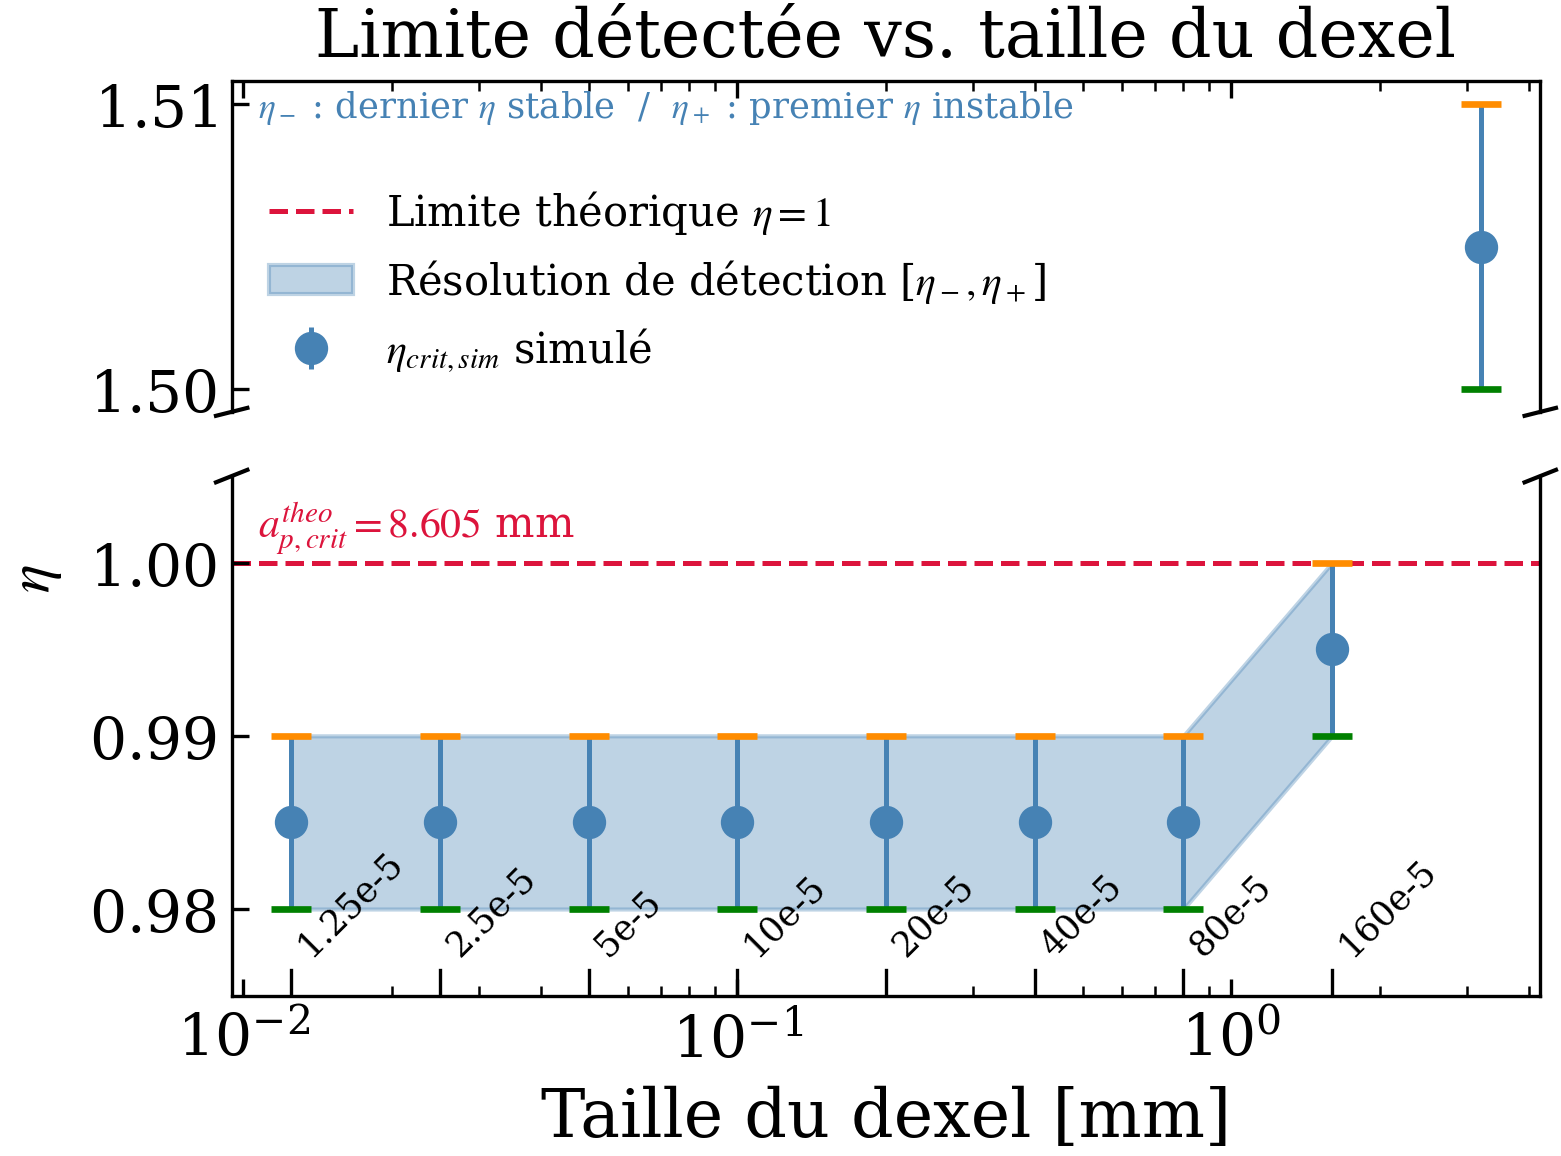
\includegraphics[width=\linewidth]{etapa2_convergence_epsilon_vs_dxl}
    \caption{Limite de stabilité simulée normalisée \(\etac\) en fonction de la taille de
    dexel \(\dxlsize\) (échelle logarithmique), avec la bande de résolution
    \([\lambda_-,\lambda_+]\) et la référence théorique \(\eta=1\). L'axe vertical est
    scindé en deux panneaux pour séparer le dexel le plus grossier du reste du balayage,
    dont l'écart à la référence est d'un autre ordre de grandeur.}
    \label{fig-convergence}
\end{figure}

Sur les huit tailles de dexel les plus fines du balayage
(\(\dxlsize \in [1,25\times10^{-5},\ 1,6\times10^{-3}]\)~m), \(\etac\) reste compris entre
\(0,985\) et \(0,995\) (\cref{fig-convergence}), soit un écart à la référence théorique de
l'ordre de \SI{1}{\percent} à \SI{2}{\percent}. Le dexel de base retenu à l'Étape~0
(\(\dxlsize = 2\times10^{-4}\)~m) se situe dans cette plage de convergence. Pour le dexel le
plus grossier du balayage (\(\dxlsize = 3,2\times10^{-3}\)~m), \(\etac \approx 1,505\) :
l'instabilité y est détectée à une profondeur environ \SI{50}{\percent} supérieure à la
valeur théorique, très en dehors de la tendance du reste du balayage.

Le même comportement qualitatif que celui observé à l'Étape~1 est retrouvé ici : les
tailles de dexel fines à intermédiaires conduisent à une détection légèrement conservatrice
(\(\etac < 1\), instabilité détectée avant la valeur théorique), tandis que la taille de
dexel la plus grossière sous-estime nettement l'instabilité (\(\etac > 1\)). La différence
notable avec l'Étape~1 est que la convergence est atteinte rapidement du côté fin du
balayage : au-delà d'un certain raffinement, réduire davantage \(\dxlsize\) n'apporte plus
de gain significatif sur \(\etac\) au regard du coût de calcul supplémentaire qu'il
implique.

\section{Conclusion}
\label{sec-conclusion}

Dans le modèle dynamique le plus simple du pipeline (\(\ap\) constant), la limite de
stabilité simulée \(\apcritsim\) converge rapidement vers la valeur théorique \(\apcrittheo\)
lorsque la taille de dexel diminue, avec un écart de l'ordre de \SI{1}{\percent} à
\SI{2}{\percent} sur la majeure partie du balayage, y compris au dexel de base retenu à
l'Étape~0. Raffiner davantage le dexel au-delà de cette plage ne se justifie donc pas au
regard du coût de calcul supplémentaire qu'il impliquerait. Seul le dexel le plus grossier
du balayage rompt cette convergence, sous-estimant nettement l'instabilité.

Cette étape établit ainsi que, dans le modèle tube, la fiabilité du simulateur vis-à-vis de
la référence théorique est robuste à la taille de dexel sur la majeure partie de la plage
testée. Le doute initial sur la convergence du modèle -- motivé par le comportement observé
dans le modèle cône -- ne se retrouve pas ici : l'origine de la dérive observée dans le
modèle cône doit donc être recherchée ailleurs, notamment dans la discrétisation temporelle
(Étape~3) ou dans les spécificités du modèle à profondeur variable (Étape~4).

% \printbibliography

\end{document}
